\documentclass[12pt,a4paper]{article}
\usepackage[a4paper,margin=1in]{geometry}
\usepackage[T1]{fontenc}
\usepackage[utf8]{inputenc}
\usepackage{lmodern}
\usepackage{setspace}
\usepackage{hyperref}
\usepackage{booktabs}
\usepackage{longtable}
\usepackage{array}
\usepackage{enumitem}
\usepackage{xcolor}
\usepackage{listings}
\usepackage{amsmath}
\usepackage{graphicx}
\usepackage{float}

\setcounter{tocdepth}{2}

\hypersetup{
	colorlinks=true,
	linkcolor=black,
	urlcolor=black,
	pdftitle={Assignment 4 Final Technical Report},
	pdfauthor={Schemeless Team}
}

\lstdefinestyle{jsonstyle}{
	basicstyle=\ttfamily\small,
	breaklines=true,
	frame=single,
	columns=fullflexible,
	showstringspaces=false,
	keepspaces=true
}

\setlist[itemize,enumerate]{itemsep=0pt,topsep=3pt,parsep=0pt,partopsep=0pt,leftmargin=*}
\setlength\parindent{0pt}

\title{\textbf{Hybrid Database Framework: Dashboard Enhancement, Performance Evaluation \& Final System Packaging}\\[0.5em]
\large Final Technical Report for CS 432: Databases -- Assignment 4}
\author{Shardul Junagade \and Kaushal Bule \and Akash Gupta}
\date{\today\\[0.3em]
\small Repository: \href{https://github.com/Kaushal845/Database_1}{\texttt{Kaushal845/Database\_1}}\\
\small Demo Video: \href{https://iitgnacin-my.sharepoint.com/:f:/g/personal/23110297_iitgn_ac_in/IgDDmiFkmFkmR7hBAn1lU5eCAbu1oP6PjvDP1tLCpSnHi_U?e=q0TZgy}{\texttt{Link}}}

\begin{document}
\maketitle
% \onehalfspacing
\setstretch{1.1}   % tighter than 1.5

\tableofcontents
\newpage

\section{Executive Summary}
This report documents the Assignment 4 completion of our hybrid SQL--MongoDB framework. Building on Assignments 1--3, our goal in this final phase was to deliver a complete and usable logical data system with three outcomes:
\begin{itemize}
	\item a dashboard that supports operational visibility without exposing backend implementation details,
	\item a benchmark suite that measures ingestion, query, metadata, and transaction behavior,
	\item a comparative study that quantifies the cost and value of abstraction versus direct database access.
\end{itemize}

Our final implementation includes an enhanced React dashboard, benchmark automation scripts, generated technical reports, and reproducible packaging through both local setup and Docker-based deployment.

\section{Project Objective and Scope}
Assignment 4 required four phases: dashboard enhancement, performance benchmarking, comparative evaluation, and deployable packaging. The scope we implemented is summarized below.

\subsection{What Was Completed}
\begin{itemize}
	\item Dashboard enhancement with dedicated tabs for logical entity exploration, query execution, query history, and performance analytics.
	\item Experimental benchmarking with persisted machine-readable outputs and formatted markdown reports.
	\item Comparative framework-versus-direct benchmarks across retrieval, nested document access, updates, and insertion.
	\item System packaging with Docker Compose and documented local setup workflows.
\end{itemize}

\subsection{Primary Deliverables Produced}
\begin{itemize}
	\item Source code repository with Assignment 4 features integrated.
	\item Performance and comparative benchmark scripts plus generated artifacts.
	\item Final dashboard with performance visualizations.
	\item Deployment and execution documentation.
\end{itemize}

\section{System Overview}
The framework exposes a logical data layer on top of two physical backends (SQLite and MongoDB). The system is metadata-driven and operation-centric:
\begin{enumerate}
	\item Ingestion pipeline classifies and routes fields.
	\item Metadata store persists placement and schema evolution decisions.
	\item Query engine accepts logical CRUD requests and executes backend-specific plans.
	\item Transaction coordinator enforces atomic cross-backend behavior via two-phase commit when enabled.
	\item Dashboard API serves logical summaries, entities, records, session activity, query history, and benchmark outputs.
\end{enumerate}

This architecture preserves abstraction for application developers while still allowing measurable, explainable execution across heterogeneous storage.

\section{Dashboard Enhancement (Assignment Section 2)}

\textbf{Implemented Dashboard Capabilities:} \\
The dashboard was enhanced to satisfy all requested capabilities from Assignment 4.

\begin{longtable}{>{\raggedright\arraybackslash}p{0.30\textwidth} >{\raggedright\arraybackslash}p{0.64\textwidth}}
\toprule
\textbf{Requirement} & \textbf{Implementation Status and Evidence} \\
\midrule
Viewing active sessions & Implemented in Session view. Shows session start time, last update, duration, and activity statistics. \\
\addlinespace
Listing logical entities within a session & Implemented in Entity Catalog. Lists discovered logical entities (nested and repeating), with filters and summaries. \\
\addlinespace
Viewing instances of each entity & Implemented in Entity Catalog via instance counts per entity and aggregate counters. \\
\addlinespace
Inspecting field names and values of logical objects & Implemented across Records and Entity Catalog. Records view supports per-record field expansion; Entity Catalog includes field-level metadata and samples. \\
\addlinespace
Displaying results of executed logical queries & Implemented in Query Builder with full CRUD execution and rendered JSON result payloads. \\
\addlinespace
Viewing query execution history & Implemented in Query History with timestamp, operation, filters, latency, status, and record counts, plus summary metrics and clear-history action. \\
\bottomrule
\end{longtable}

\textbf{Constraint Compliance: Logical View Without Backend Leakage} \\
The assignment constraint requires that users interact with logical abstractions rather than physical storage details. We reviewed and adjusted UI wording so regular dashboard views avoid exposing implementation-level terms like SQL table names, MongoDB collection names, index internals, or placement internals.

Technical comparative views (Performance tab) intentionally mention direct SQL and MongoDB because Assignment 4 Sections 3 and 4 explicitly require that comparison.

\textbf{Dashboard Screenshots:}
\begin{figure}[H]
\centering
% \fbox{\parbox{0.90\textwidth}{\vspace{2.8cm}
% \centering\textbf{Placeholder: Screenshot A -- Query History Tab}\\
% Include filters, latency colors, success/failure counts, and recent query table.\\
% \vspace{2.8cm}}}
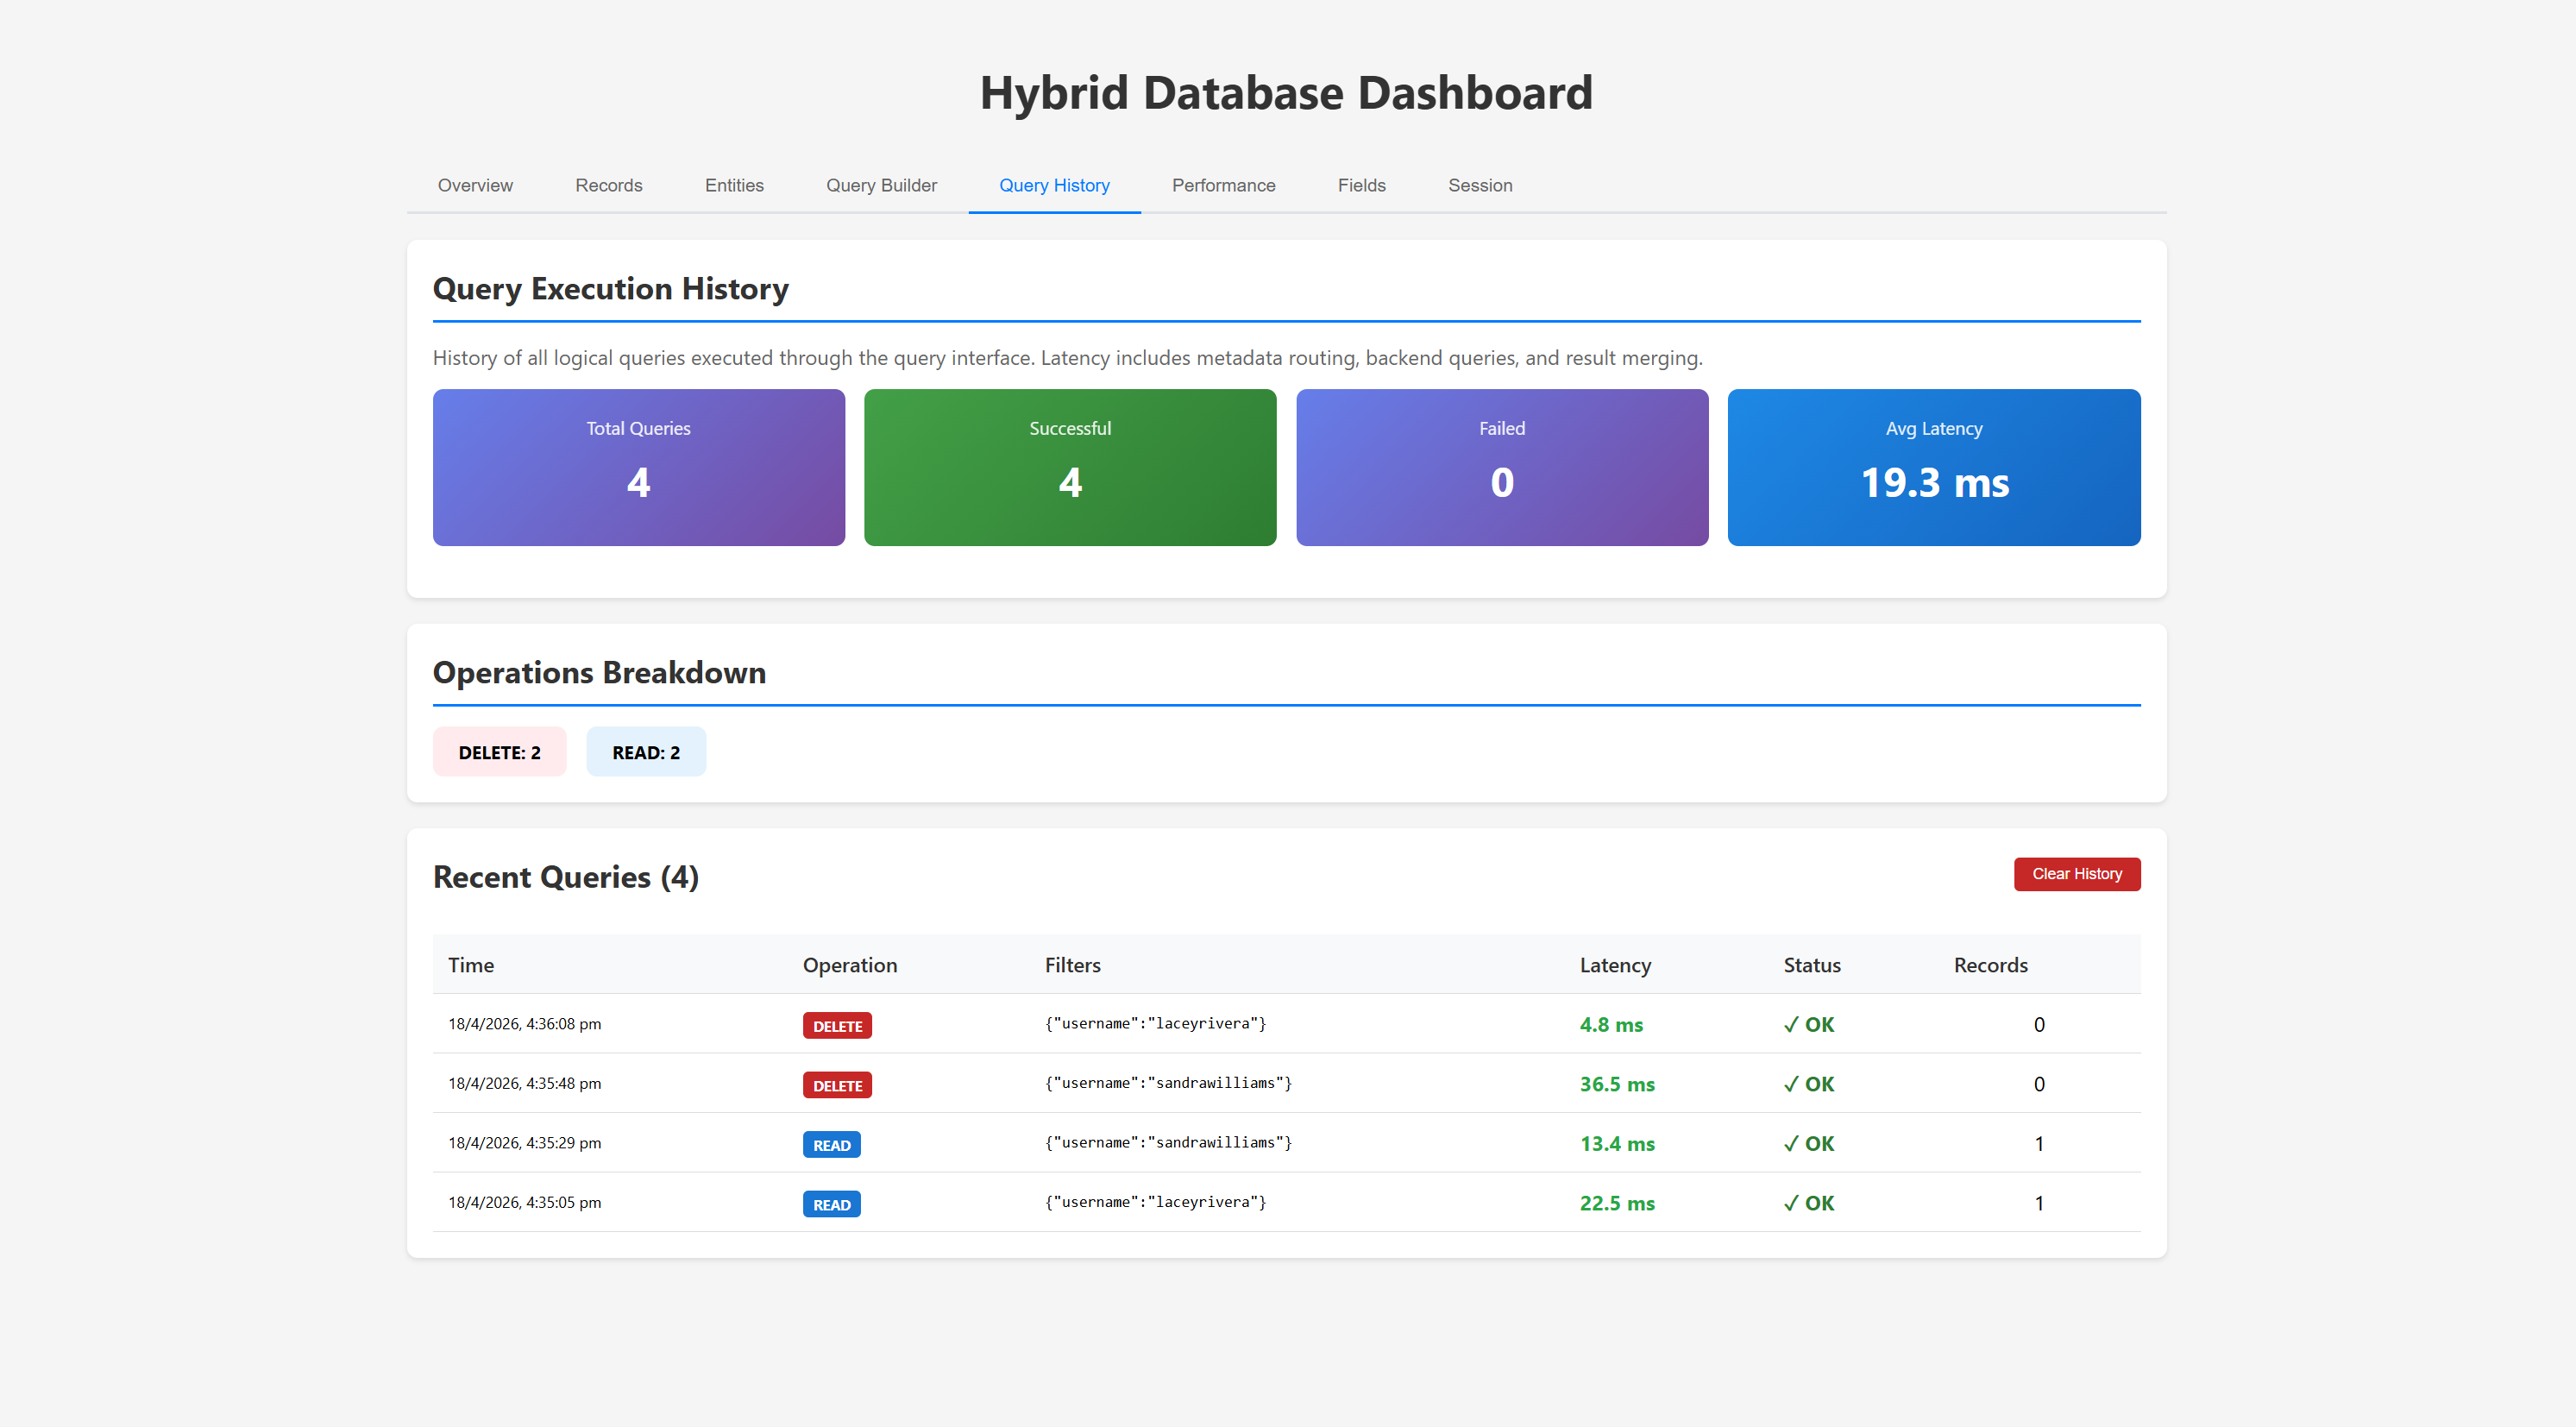
\includegraphics[width=0.90\textwidth]{images/A4/query_history.png}
\caption{Query execution history in the enhanced dashboard.}
\end{figure}

\begin{figure}[H]
\centering
% \fbox{\parbox{0.90\textwidth}{\vspace{2.8cm}
% \centering\textbf{Placeholder: Screenshot B -- Performance Tab}\\
% Include ingestion chart, query chart, transaction overhead chart, and summary table.\\
% \vspace{2.8cm}}}
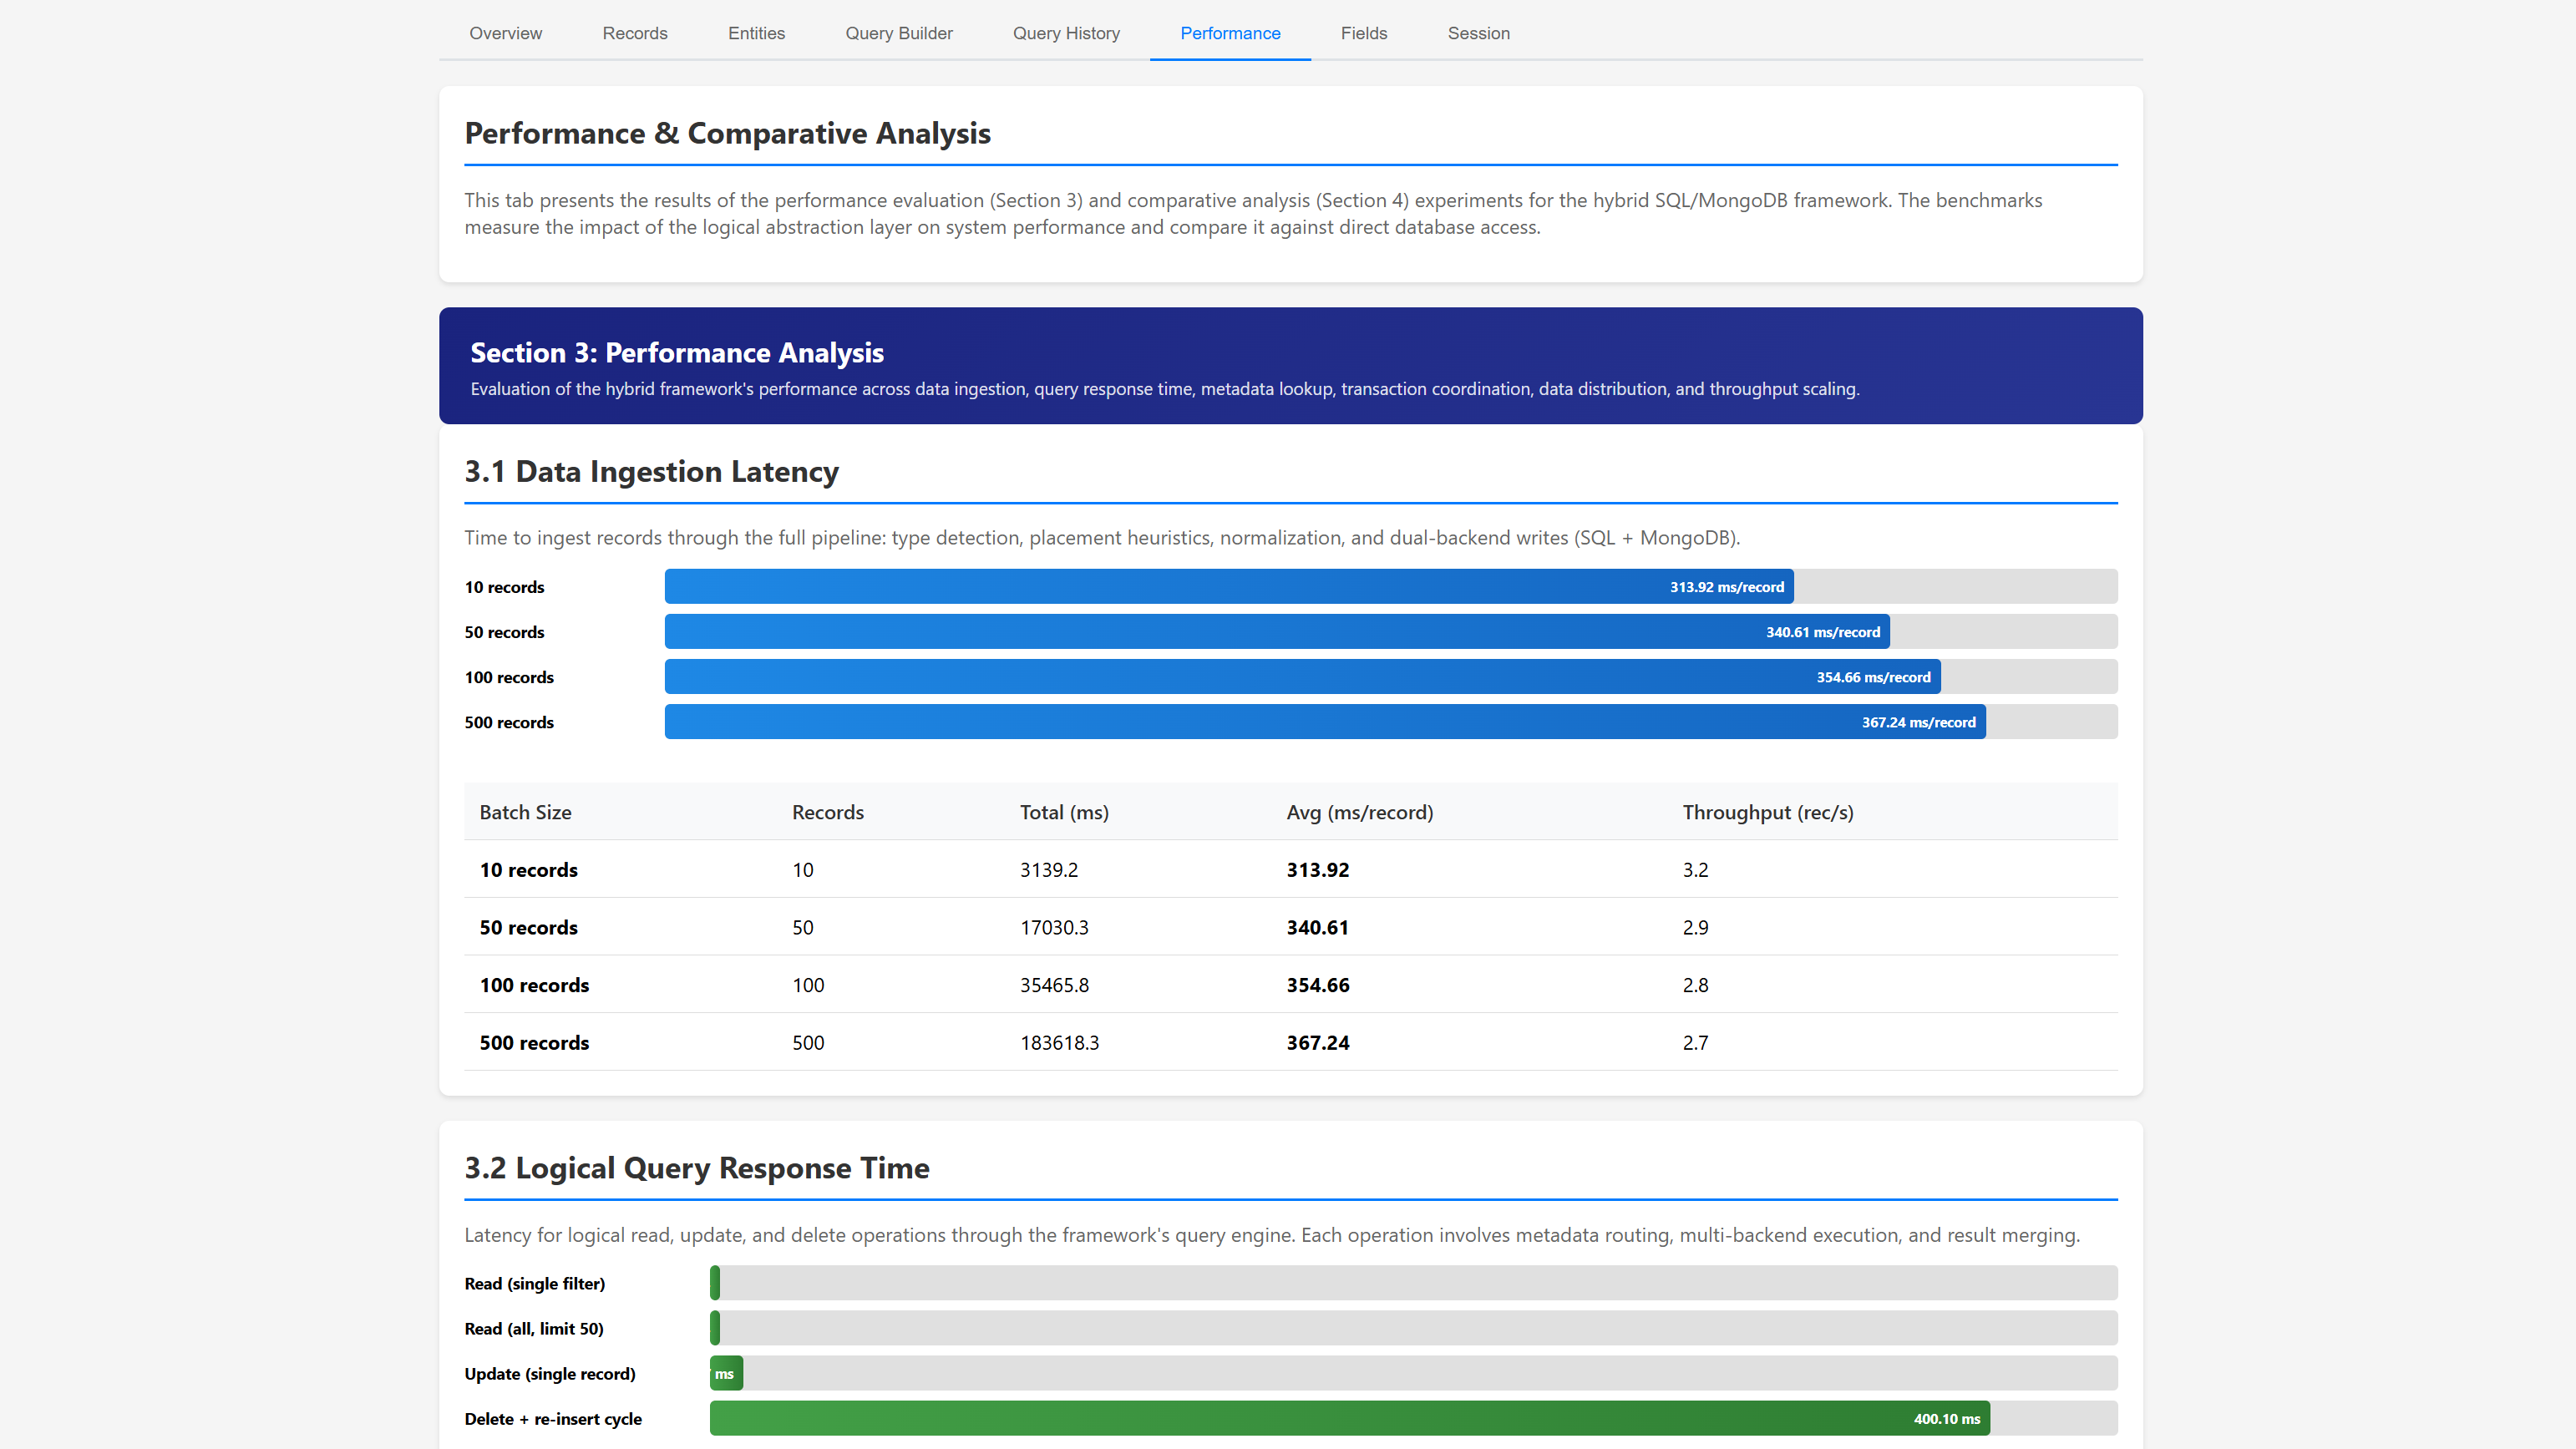
\includegraphics[width=0.90\textwidth]{images/A4/performance_tab.png}
\caption{Performance analytics integrated into the dashboard.}
\end{figure}

\begin{figure}[H]
\centering
% \fbox{\parbox{0.90\textwidth}{\vspace{2.8cm}
% \centering\textbf{Placeholder: Screenshot C -- Entity Catalog and Record Inspector}\\
% Show logical entities, per-entity counts, and expanded field/value inspection.\\
% \vspace{2.8cm}}}
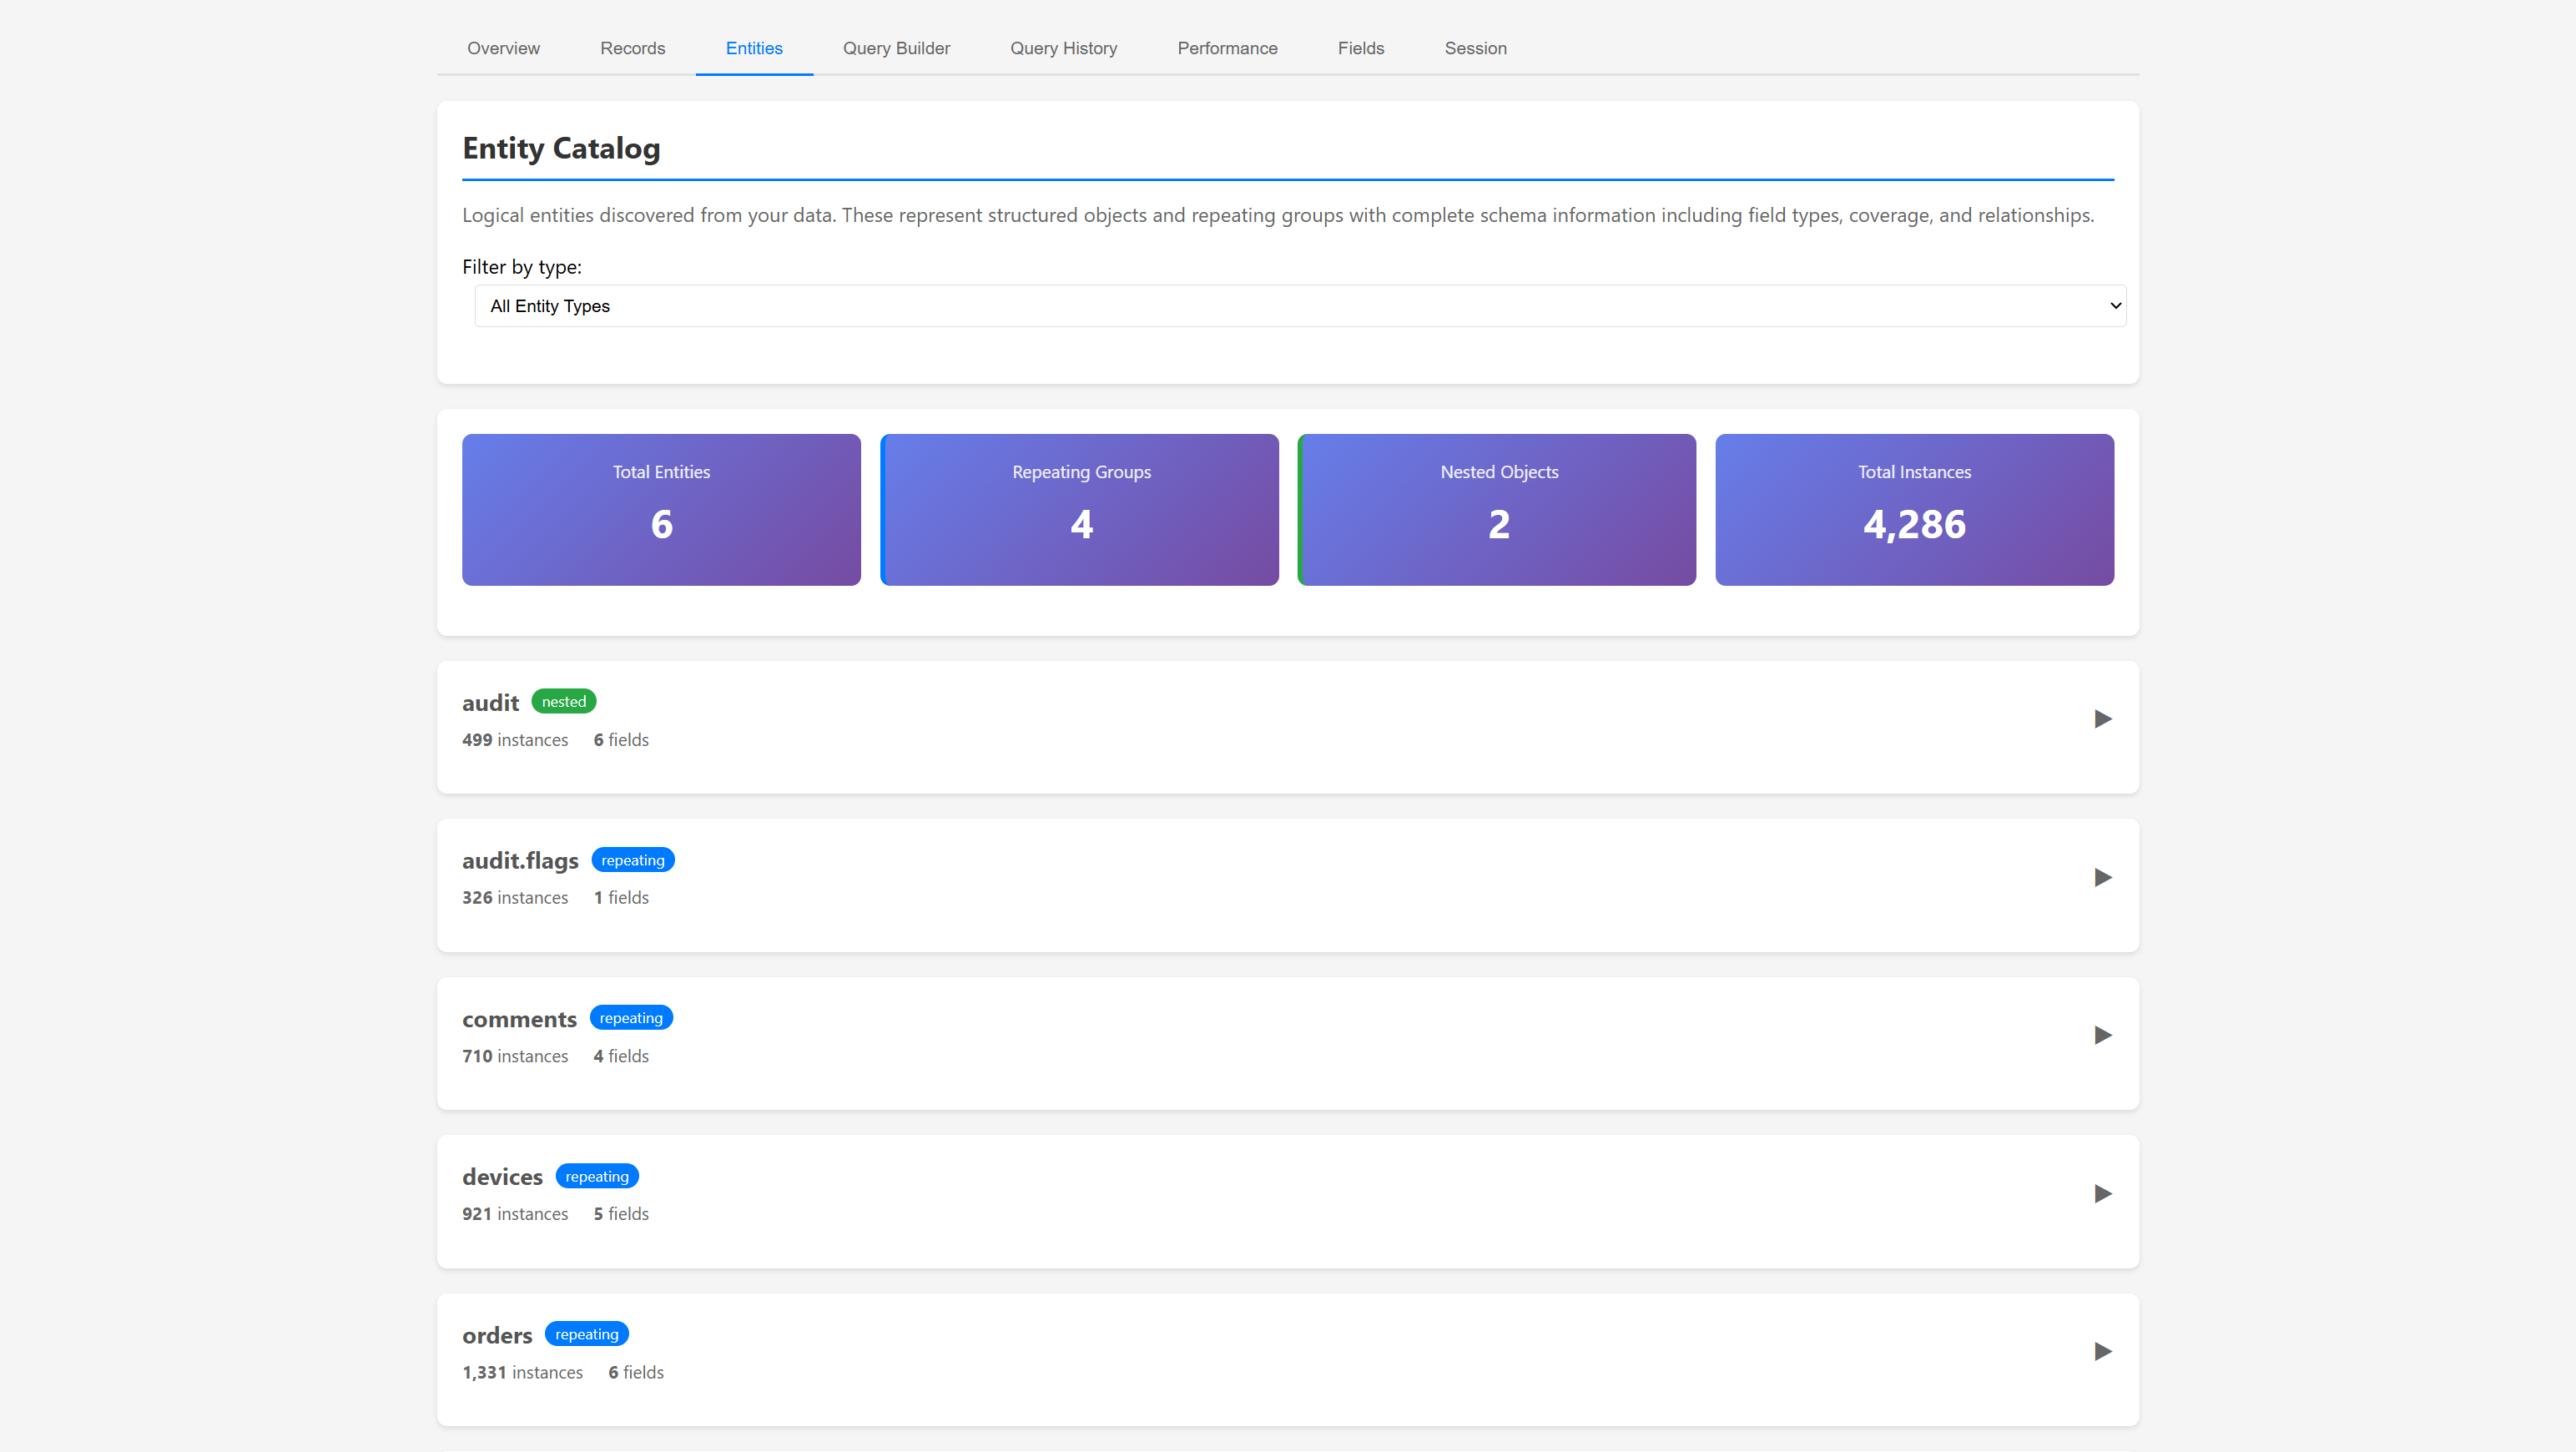
\includegraphics[width=0.90\textwidth]{images/A4/entity_catalog.png}
\caption{Entity catalog view in the enhanced dashboard.}
\end{figure}

\begin{figure}[H]
\centering
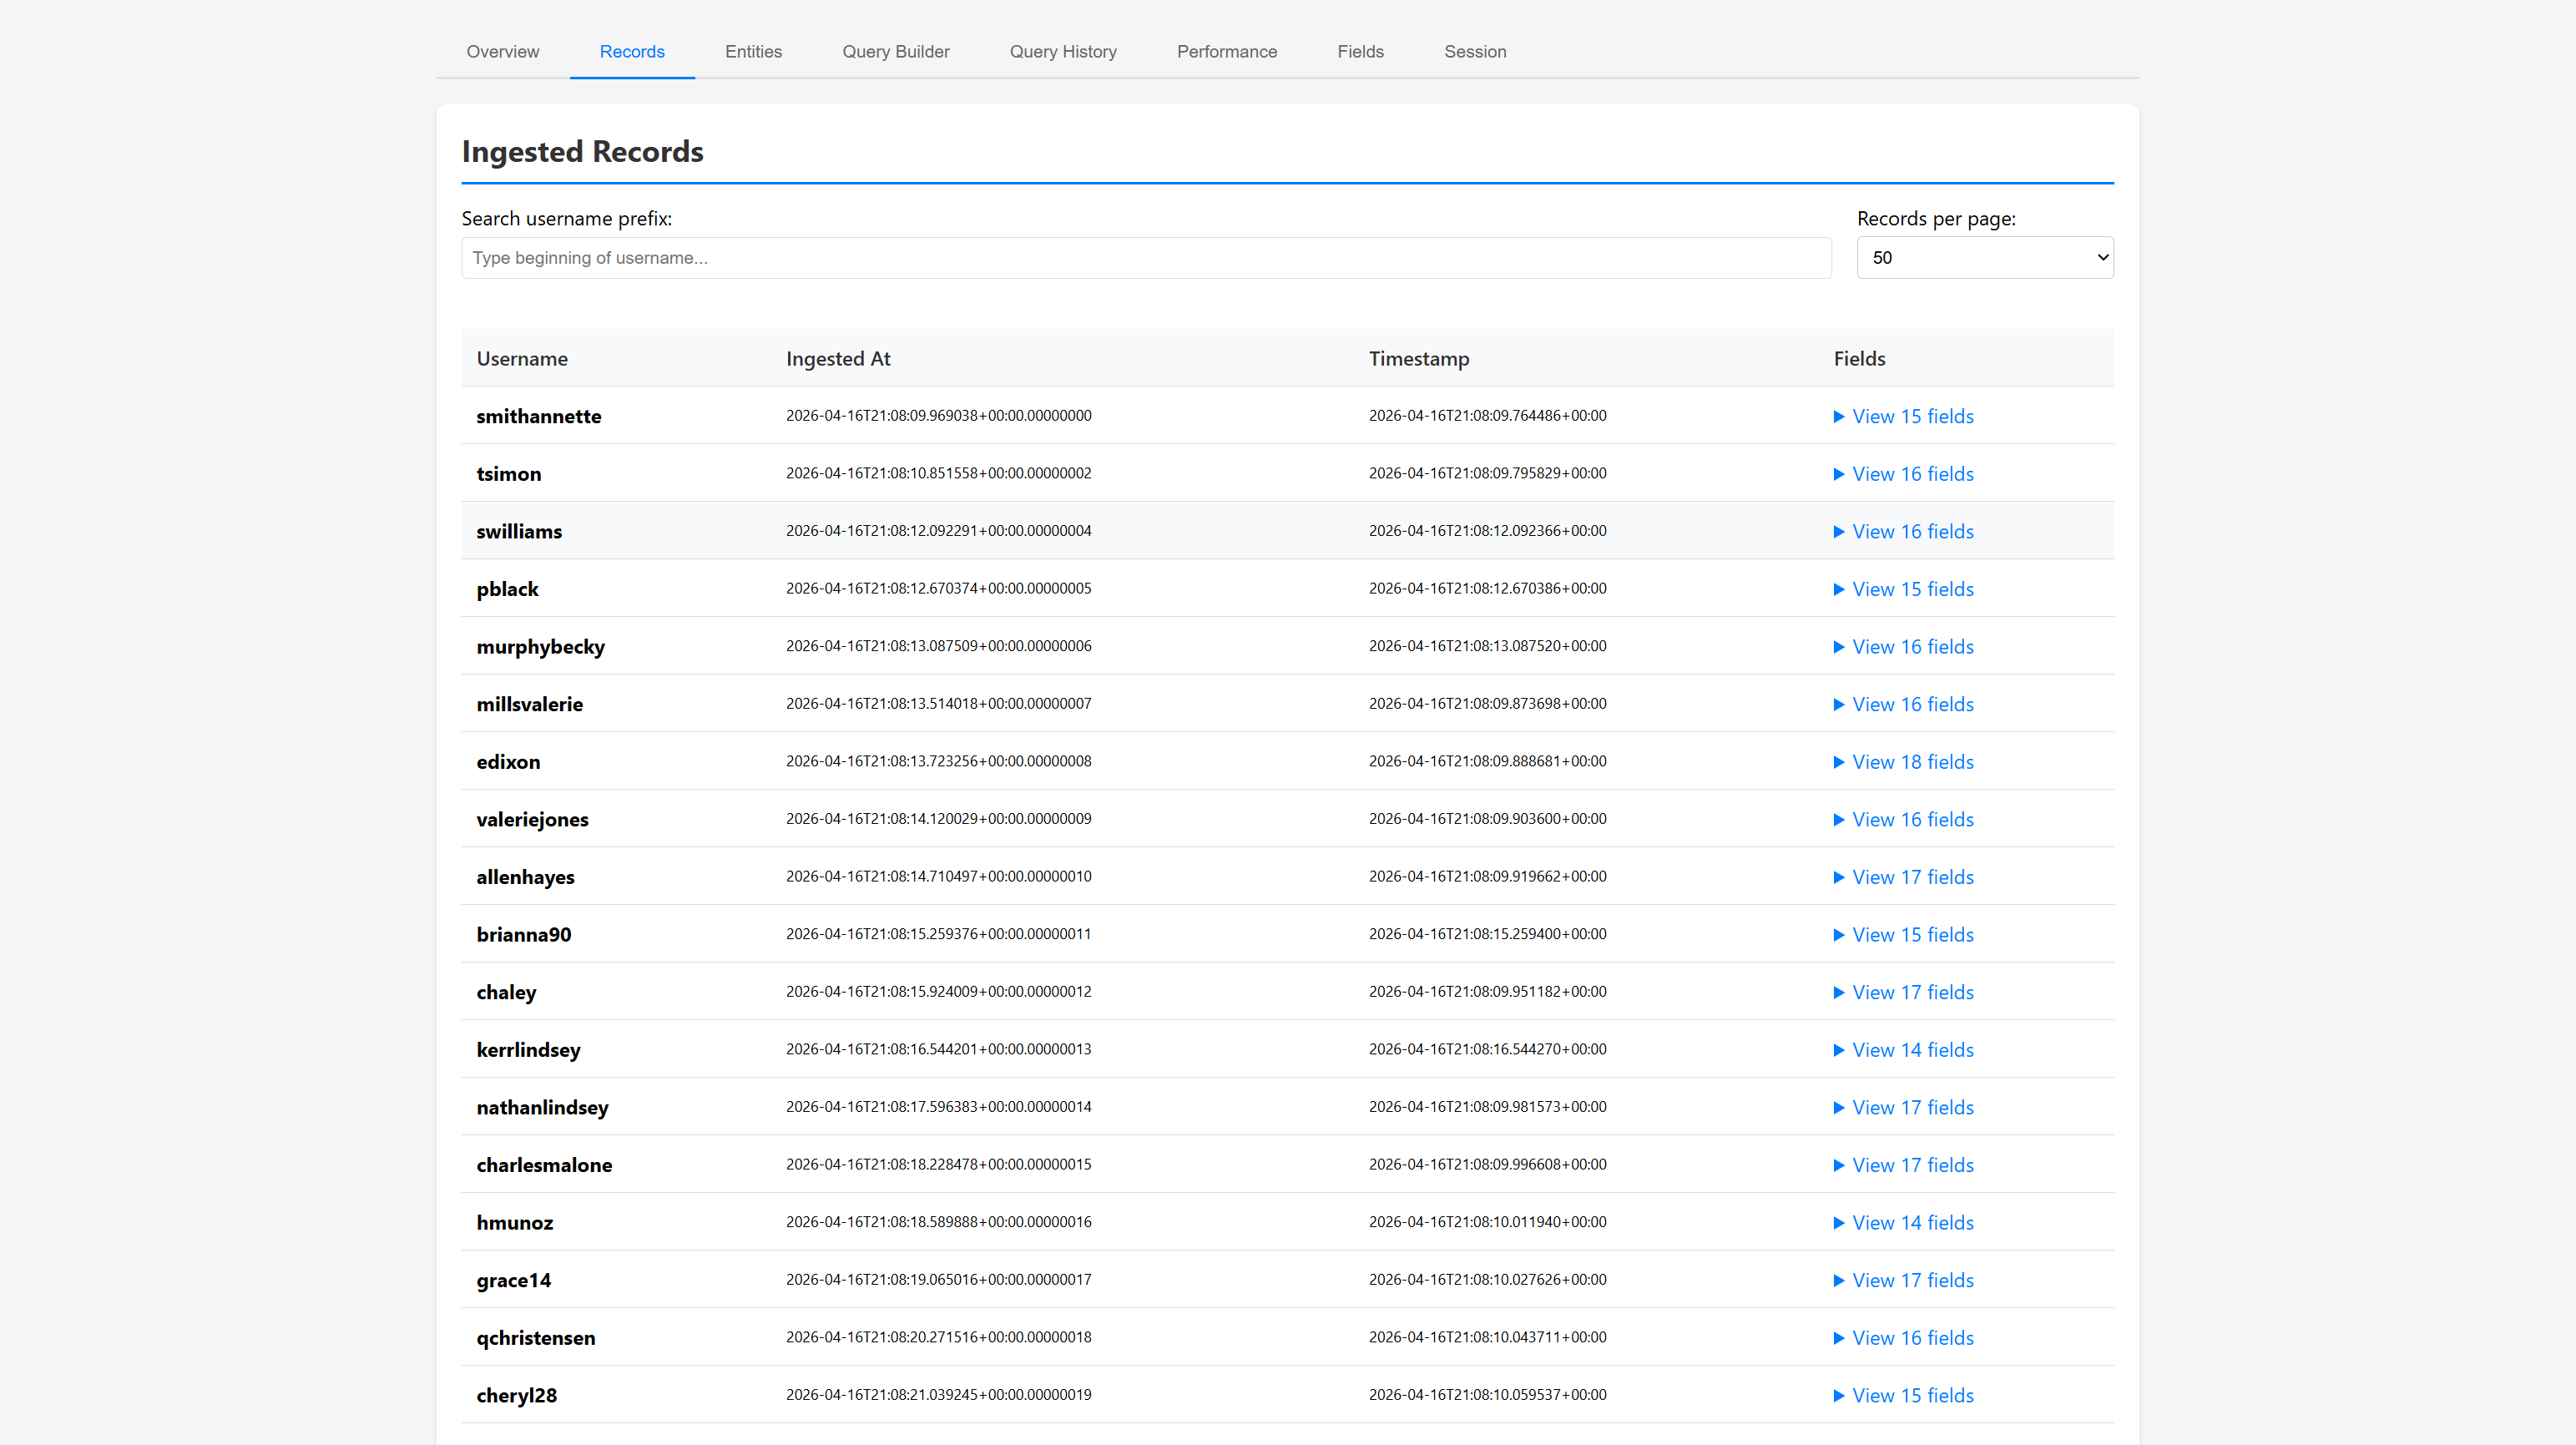
\includegraphics[width=0.90\textwidth]{images/A4/record_inspector.png}
\caption{Record inspector view in the enhanced dashboard.}
\end{figure}

\section{Performance Evaluation (Assignment Section 3)}

\subsection{Experimental Design}
To evaluate the hybrid framework, we implemented a repeatable benchmark suite focused on assignment-mandated dimensions:
\begin{itemize}
	\item data ingestion latency,
	\item logical query response time,
	\item metadata lookup overhead,
	\item transaction coordination overhead across SQL and MongoDB.
\end{itemize}

In addition, we collected:
\begin{itemize}
	\item average query latency and tail metrics,
	\item throughput in operations per second,
	\item distribution of fields and records across backends.
\end{itemize}

\subsection{Environment and Dataset}
\begin{itemize}
	\item Data generator: Faker-based synthetic records with scalar fields and nested structures.
	\item Backends: SQLite (embedded) and MongoDB.
	\item Runtime: Python 3.13.7.
	\item Seed size for query benchmarks: 100 records.
\end{itemize}

\textbf{Note:} Replace with machine details before final PDF export.
\begin{itemize}
	\item CPU: \textbf{Intel i7-13700H}
	\item RAM: \textbf{16 GB}
	\item OS: \textbf{Windows 11}
\end{itemize}

\subsection{Performance Results}

Execution of benchmark suites generating:
\begin{itemize}
    \item \texttt{docs/performance\_benchmark\_results.json},
    \item \texttt{docs/comparative\_benchmark\_results.json},
    \item \texttt{docs/performance\_report.md},
    \item \texttt{docs/comparative\_report.md}.
\end{itemize}

\subsubsection{Ingestion Latency and Throughput}
\begin{table}[H]
\centering
\begin{tabular}{r r r r}
\toprule
\textbf{Batch Size} & \textbf{Total (ms)} & \textbf{Avg (ms/record)} & \textbf{Throughput (rec/s)} \\
\midrule
10 & 3139.2 & 313.924 & 3 \\
50 & 17030.3 & 340.605 & 3 \\
100 & 35465.8 & 354.658 & 3 \\
500 & 183618.3 & 367.237 & 3 \\
\bottomrule
\end{tabular}
\caption{Ingestion benchmark results.}
\end{table}

\subsubsection{Logical Query Response Time}
\begin{table}[H]
\centering
\begin{tabular}{l r r r r r}
\toprule
\textbf{Operation} & \textbf{Avg (ms)} & \textbf{Min (ms)} & \textbf{Max (ms)} & \textbf{P95 (ms)} & \textbf{Iters} \\
\midrule
Read (single filter) & 1.72 & 1.16 & 5.35 & 2.87 & 50 \\
Read (all, limit 50) & 3.05 & 1.85 & 5.53 & 4.55 & 30 \\
Update (single record) & 10.47 & 2.87 & 21.68 & 17.79 & 30 \\
Delete + re-insert cycle & 400.10 & 255.11 & 816.63 & 702.26 & 20 \\
\bottomrule
\end{tabular}
\caption{Logical query latency across operations.}
\end{table}

\subsubsection{Metadata Lookup Overhead}
\begin{table}[H]
\centering
\begin{tabular}{l r r}
\toprule
\textbf{Operation} & \textbf{Avg (ms)} & \textbf{Iterations} \\
\midrule
Field mapping lookup & 0.0001 & 200 \\
Placement decision lookup & 0.0001 & 200 \\
\bottomrule
\end{tabular}
\caption{Metadata lookup overhead.}
\end{table}

\subsubsection{Transaction Coordination Overhead}
\begin{table}[H]
\centering
\begin{tabular}{l r r}
\toprule
\textbf{Operation} & \textbf{Avg (ms)} & \textbf{Iterations} \\
\midrule
Full 2PC (begin $\rightarrow$ prepare $\rightarrow$ commit) & 2.44 & 20 \\
Direct update (no 2PC) & 2.75 & 20 \\
\bottomrule
\end{tabular}
\caption{2PC coordination overhead versus direct update.}
\end{table}

\subsubsection{Data Distribution Across Backends}
\begin{table}[H]
\centering
\begin{tabular}{l r}
\toprule
\textbf{Backend} & \textbf{Fields Stored} \\
\midrule
SQL & 3 \\
MongoDB & 7 \\
Both & 1 \\
Buffer & 0 \\
\textbf{Total} & \textbf{8} \\
\bottomrule
\end{tabular}
\caption{Field distribution across storage backends.}
\end{table}

\begin{table}[H]
\centering
\begin{tabular}{l r}
\toprule
\textbf{Storage} & \textbf{Record Count} \\
\midrule
SQL (main table) & 100 \\
MongoDB (main collection) & 100 \\
Buffer (pending) & 0 \\
\bottomrule
\end{tabular}
\caption{Record distribution across storage objects.}
\end{table}

\subsubsection{Throughput Under Increasing Workload}
\begin{table}[H]
\centering
\begin{tabular}{r r r}
\toprule
\textbf{Workload (ops)} & \textbf{Elapsed (s)} & \textbf{Throughput (ops/s)} \\
\midrule
10 & 0.027 & 372.1 \\
25 & 0.089 & 281.6 \\
50 & 0.118 & 423.7 \\
100 & 0.372 & 268.7 \\
\bottomrule
\end{tabular}
\caption{Read throughput scaling.}
\end{table}

\subsection{Interpretation of Performance Results}
The measurements are consistent with a metadata-driven, dual-write architecture:
\begin{itemize}
	\item Ingestion cost remains the dominant write overhead because one logical write can trigger classification, metadata updates, normalization handling, and writes to two backends.
	\item Query latency stays low in absolute terms for this dataset size; however, update and delete+reinsert costs are higher due to coordination and consistency workflows.
	\item Metadata lookups are effectively negligible relative to query and ingest costs.
	\item Throughput trends are broadly stable under moderate read load, indicating practical scalability for assignment-scale workloads.
\end{itemize}

\section{Comparative Analysis (Assignment Section 4)}

\subsection{Comparative Experiment Design}
We compared logical framework operations against direct backend access to quantify abstraction cost and benefit. The implemented comparisons were:
\begin{enumerate}
	\item Record retrieval: framework read vs direct SQL SELECT vs direct MongoDB find.
	\item Nested document access: framework read vs direct MongoDB find with projection.
	\item Record update: framework logical update vs direct SQL UPDATE vs direct MongoDB \$set.
	\item Record insertion: framework ingest vs direct SQL INSERT vs direct MongoDB insert\_one.
\end{enumerate}

\subsection{Comparative Results (Measured)}
\begin{table}[H]
\centering
\begin{tabular}{l r r r r}
\toprule
\textbf{Test} & \textbf{Framework (ms)} & \textbf{Direct SQL (ms)} & \textbf{Direct MongoDB (ms)} & \textbf{Overhead} \\
\midrule
Record Retrieval (single filter read) & 2.40 & 0.02 & 1.16 & 103.0\% \\
Nested Document Access (orders + profile) & 3.36 & N/A & 1.49 & 126.1\% \\
Record Update (single field) & 8.81 & 0.02 & 1.20 & 619.0\% \\
Record Insertion & 366.77 & 0.10 & 1.03 & 32214.4\% \\
\bottomrule
\end{tabular}
\caption{Comparative summary (framework vs direct access).}
\end{table}

\subsection{Detailed Per-Test Latency Tables}
\subsubsection{Record Retrieval}
\begin{table}[H]
\centering
\begin{tabular}{l r r r r}
\toprule
\textbf{Method} & \textbf{Avg (ms)} & \textbf{Min (ms)} & \textbf{Max (ms)} & \textbf{P95 (ms)} \\
\midrule
Framework (logical query) & 2.403 & 1.885 & 3.899 & 3.088 \\
Direct SQL (SELECT) & 0.023 & 0.020 & 0.080 & 0.025 \\
Direct MongoDB (find) & 1.161 & 0.705 & 1.800 & 1.561 \\
\bottomrule
\end{tabular}
\caption{Record retrieval latency breakdown.}
\end{table}

\subsubsection{Nested Document Access}
\begin{table}[H]
\centering
\begin{tabular}{l r r r r}
\toprule
\textbf{Method} & \textbf{Avg (ms)} & \textbf{Min (ms)} & \textbf{Max (ms)} & \textbf{P95 (ms)} \\
\midrule
Framework (logical query) & 3.362 & 2.233 & 5.619 & 4.853 \\
Direct MongoDB (find + projection) & 1.487 & 1.131 & 3.045 & 2.028 \\
\bottomrule
\end{tabular}
\caption{Nested document access latency breakdown.}
\end{table}

\subsubsection{Record Update}
\begin{table}[H]
\centering
\begin{tabular}{l r r r r}
\toprule
\textbf{Method} & \textbf{Avg (ms)} & \textbf{Min (ms)} & \textbf{Max (ms)} & \textbf{P95 (ms)} \\
\midrule
Framework (logical update) & 8.815 & 6.511 & 16.013 & 11.075 \\
Direct SQL (UPDATE) & 0.022 & 0.014 & 0.209 & 0.017 \\
Direct MongoDB (\$set) & 1.204 & 0.914 & 1.627 & 1.582 \\
\bottomrule
\end{tabular}
\caption{Record update latency breakdown.}
\end{table}

\subsubsection{Record Insertion}
\begin{table}[H]
\centering
\begin{tabular}{l r r r r}
\toprule
\textbf{Method} & \textbf{Avg (ms)} & \textbf{Min (ms)} & \textbf{Max (ms)} & \textbf{P95 (ms)} \\
\midrule
Framework (full pipeline) & 366.768 & 274.711 & 1237.725 & 372.490 \\
Direct SQL (INSERT) & 0.103 & 0.067 & 0.270 & 0.182 \\
Direct MongoDB (insert\_one) & 1.032 & 0.560 & 1.645 & 1.567 \\
\bottomrule
\end{tabular}
\caption{Record insertion latency breakdown.}
\end{table}

\subsection{4.6 Discussion: Overhead vs Value}

\subsubsection*{Where the abstraction adds overhead}
\begin{itemize}
	\item \textbf{Read operations}: The framework performs metadata lookups, routes queries to both SQL and MongoDB, and merges results. This adds measurable latency compared to a single direct query.
	\item \textbf{Ingestion}: The framework runs type detection, placement heuristics, normalization, and dual-backend writes, which is significantly slower than a single raw INSERT.
	\item \textbf{Updates}: The framework routes fields to the correct backend based on metadata, potentially updating SQL and MongoDB separately. Direct updates on a single backend are naturally faster.
\end{itemize}

\subsubsection*{Where the abstraction provides value}
\begin{itemize}
	\item \textbf{Unified access}: Users query a single logical interface without knowing which backend stores each field.
	\item \textbf{Automatic schema evolution}: New fields are automatically detected, classified, and routed to an appropriate backend.
	\item \textbf{Nested entity management}: Arrays can be normalized into child tables while embedded documents remain document-native in MongoDB, all transparently.
	\item \textbf{ACID guarantees}: The two-phase commit model provides atomic behavior across both backends.
	% \item \textbf{Backend-agnostic applications}: Application logic does not need to change when placement decisions evolve.
\end{itemize}

\subsubsection*{When to use framework vs direct access}
\begin{table}[H]
\centering
\begin{tabular}{l l}
\toprule
\textbf{Scenario} & \textbf{Recommended Approach} \\
\midrule
Schema-flexible, evolving data & Framework \\
High-throughput, fixed-schema writes & Direct backend \\
Cross-backend queries (SQL + MongoDB) & Framework \\
Single-backend, latency-critical reads & Direct backend \\
Need ACID across SQL + MongoDB & Framework \\
\bottomrule
\end{tabular}
\caption{Decision guide: abstraction layer vs direct backend access.}
\end{table}


\section{Final System Packaging (Assignment Section 5)}

\subsection{Reproducible Setup Paths}
The framework is packaged with two setup strategies to support different evaluator environments:
\begin{itemize}
	\item \textbf{Docker-based setup} for one-command reproducibility,
	\item \textbf{Local setup} for development and debugging.
\end{itemize}

\subsection{Packaging Components Delivered}
\begin{longtable}{>{\raggedright\arraybackslash}p{0.32\textwidth} >{\raggedright\arraybackslash}p{0.62\textwidth}}
\toprule
\textbf{Required Item} & \textbf{What is Provided} \\
\midrule
Source code repository & GitHub repository with backend, frontend, benchmark scripts, tests, and docs. \\
Setup instructions for dependencies & Python and Node dependency docs, runnable command references. \\
SQL and MongoDB configuration guidance & SQLite defaults documented; MongoDB local and Docker startup documented. \\
Run ingestion API instructions & API startup and ingestion flow documented. \\
Run logical query interface instructions & Query Builder and API endpoint workflows documented. \\
Launch dashboard instructions & Local frontend workflow and Docker integrated dashboard workflow documented. \\
\bottomrule
\end{longtable}

\subsection{Docker Packaging Summary}
Using \texttt{docker compose up --build} starts:
\begin{itemize}
	\item MongoDB container,
	\item App container serving FastAPI and built dashboard.
\end{itemize}

Exposed endpoints include dashboard UI, API docs, and health endpoint. The Docker guide also includes ingestion commands, query examples, benchmark execution commands, and TA demonstration flow.

\textbf{Deployment and API Evidence Screenshots:}
\begin{figure}[H]
\centering
% \fbox{\parbox{0.90\textwidth}{\vspace{2.6cm}
% \centering\textbf{Placeholder: Docker Deployment Screenshot}\\
% Add screenshot of \texttt{docker compose ps} and/or health output.\\
% \vspace{2.6cm}}}
% Replace placeholder with actual image command:
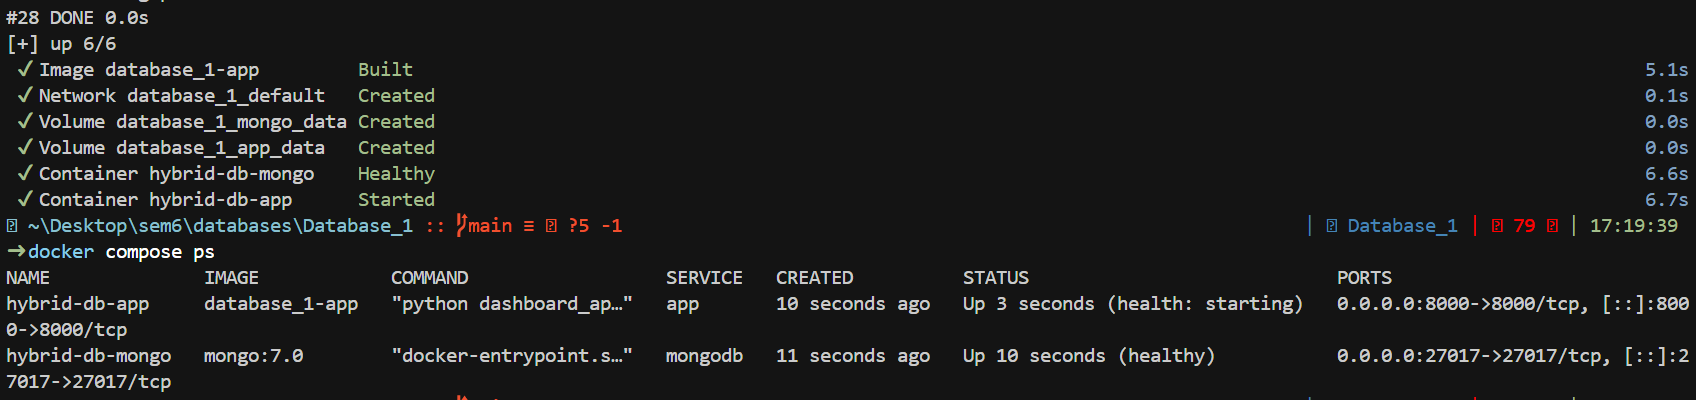
\includegraphics[width=0.90\textwidth]{images/A4/docker_deploy.png}
\caption{Dockerized deployment.}
\end{figure}

\begin{figure}[H]
\centering
% \fbox{\parbox{0.90\textwidth}{\vspace{2.6cm}
% \centering\textbf{Placeholder: Endpoint Response Screenshot}\\
% Add screenshot of benchmark endpoint JSON or a read endpoint response.\\
% \vspace{2.6cm}}}
% Replace placeholder with actual image command:
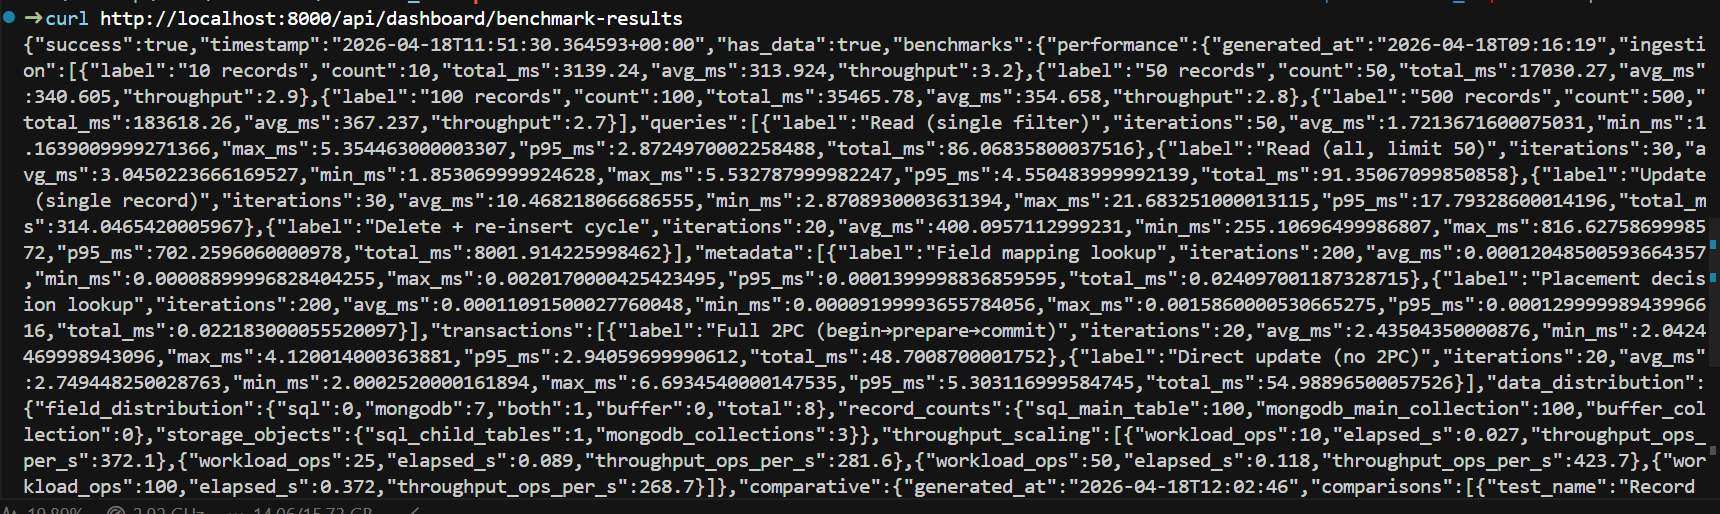
\includegraphics[width=0.90\textwidth]{images/A4/benchmark_endpoint.png}
\caption{API evidence from benchmark endpoint output.}
\end{figure}

\section{Summary of Assignment Requirements}
\begin{longtable}{>{\raggedright\arraybackslash}p{0.24\textwidth} >{\raggedright\arraybackslash}p{0.70\textwidth}}
\toprule
\textbf{Criterion} & \textbf{Coverage in This Submission} \\
\midrule
Dashboard Enhancement & Usable and logically-oriented multi-tab dashboard with session tracking, entity catalog, record inspection, query execution, and query history, while preserving abstraction constraints in core views. \\
\addlinespace
Performance Evaluation & Dedicated benchmark suite with ingestion, query, metadata, transaction, throughput, and distribution measurements; includes reproducible script outputs and interpretation. \\
\addlinespace
Comparative Analysis & Framework-vs-direct benchmarks for retrieval, nested access, updates, insertion; latency and overhead tables plus trade-off discussion and usage recommendations. \\
\addlinespace
System Packaging & Complete local and Docker setup instructions, service map, run commands, and demonstration flow for fast evaluator onboarding. \\
\addlinespace
Report Quality & Structured technical narrative with data tables, interpretation, constraints, limitations, and checklist-driven evidence mapping to assignment requirements. \\
\bottomrule
\end{longtable}

\section{Limitations}
\begin{itemize}
	\item Some percentage-overhead values can look unintuitive when direct baseline latency is extremely small.
	\item Current deployment is single-node and primarily optimized for coursework-scale data volumes.
\end{itemize}

% \subsection{Planned Improvements}
% \begin{itemize}
% 	\item Add normalized overhead metrics (for example, against combined baseline or geometric mean baseline) for more interpretable comparative reporting.
% 	\item Add automated generation of publication-grade charts directly into the report artifacts.
% 	\item Expand workload scenarios for concurrent read/write stress and long-running ingestion sessions.
% \end{itemize}

\section{Conclusion}

Assignment 4 transformed the project from a prototype data pipeline into a complete logical data platform with measurable behavior and reproducible execution. The dashboard now supports end-user observability and interaction, benchmarks quantify system costs and behavior, comparative analysis explains the abstraction trade-offs, and packaging enables straightforward deployment.

In short, the final system demonstrates the practical value of a metadata-driven logical layer over heterogeneous stores: measurable overhead exists, but so does meaningful reduction in application complexity, improved evolvability, and stronger consistency guarantees across backends.

\end{document}
